
\documentclass[review]{elsarticle}

\usepackage{lineno,hyperref}
\usepackage[mathletters]{ucs}
\usepackage[utf8x]{inputenc}
\usepackage{algorithm,algorithmic}% http://ctan.org/pkg/algorithms
\usepackage{natbib}
\usepackage{supertabular}
\usepackage{fancybox}
\usepackage{acronym}
\usepackage{array}
\usepackage{booktabs}
\usepackage{graphicx}
\usepackage{rotating}
\usepackage{tabularx}
\usepackage{colortbl}
\usepackage{multirow}
\usepackage{hhline}
\usepackage{setspace}
\usepackage{placeins}
\usepackage{longtable}
\usepackage{mathtools}
\usepackage{listings}
\usepackage{epstopdf}
\usepackage{subfigure}
\usepackage{courier}
\usepackage{amsfonts}
\usepackage{morefloats}
\usepackage{lipsum}
\usepackage{amsthm,amsmath}

% declarations
\DeclarePairedDelimiter\abs{\lvert}{\rvert}%
\DeclarePairedDelimiter\norm{\lVert}{\rVert}%
\DeclareMathOperator*{\argmin}{arg\,min}
\DeclareMathOperator*{\argmax}{arg\,max}
\newcommand*\justify{%
	\fontdimen2\font=0.4em% interword space
	\fontdimen3\font=0.2em% interword stretch
	\fontdimen4\font=0.1em% interword shrink
	\fontdimen7\font=0.1em% extra space
	%\hyphenchar\font=`\-% allowing hyphenation
}

% table
\usepackage{color, colortbl}
\definecolor{Gray}{gray}{0.9}

% Algorithmic modifications
\makeatletter
\newcommand{\ALOOP}[1]{\ALC@it\algorithmicloop\ #1%
  \begin{ALC@loop}}
\newcommand{\ENDALOOP}{\end{ALC@loop}\ALC@it\algorithmicendloop}
\renewcommand{\algorithmicrequire}{\textbf{Input:}}
\renewcommand{\algorithmicensure}{\textbf{Output:}}
\newcommand{\algorithmicbreak}{\textbf{break}}
\newcommand{\BREAK}{\STATE \algorithmicbreak}
\makeatother

% appendix
\usepackage[titletoc,title]{appendix}
\usepackage{hyperref}
\usepackage{cleveref}

\modulolinenumbers[5]

\journal{Journal of Network and Computer Applications}

%%%%%%%%%%%%%%%%%%%%%%%
%% Elsevier bibliography styles
%%%%%%%%%%%%%%%%%%%%%%%
%% To change the style, put a % in front of the second line of the current style and
%% remove the % from the second line of the style you would like to use.
%%%%%%%%%%%%%%%%%%%%%%%

%% Numbered
%\bibliographystyle{model1-num-names}

%% Numbered without titles
%\bibliographystyle{model1a-num-names}

%% Harvard
%\bibliographystyle{model2-names.bst}\biboptions{authoryear}

%% Vancouver numbered
%\usepackage{numcompress}\bibliographystyle{model3-num-names}

%% Vancouver name/year
%\usepackage{numcompress}\bibliographystyle{model4-names}\biboptions{authoryear}

%% APA style
%\bibliographystyle{model5-names}\biboptions{authoryear}

%% AMA style
%\usepackage{numcompress}\bibliographystyle{model6-num-names}

%% `Elsevier LaTeX' style
\bibliographystyle{elsarticle-num}
%%%%%%%%%%%%%%%%%%%%%%%

\begin{document}

\begin{frontmatter}

\title{Robust PCA and Higher Moments Distances for Botnet Detection}

%% Group authors per affiliation:
\author[unbaddress]{Thiago P. B. Vieira}
\author[unbaddress]{Eduardo Said Calil Vilaça}
\author[unbaddress,Ilmenauaddress,Fraunhoferaddress]{João Paulo C. L. da Costa}
\author[unbaddress]{Rafael T. de Sousa Júnior}

\address[unbaddress]{Department of Electrical Engineering, University of Brasilia (UnB), 70910-900, Brasília-DF, Brazil}
\address[Ilmenauaddress]{Institute for Information Technology, Ilmenau University of Technology, Ilmenau, Germany}
\address[Fraunhoferaddress]{Fraunhofer Institute for Integrated Circuits IIS, Erlangen, Germany}


\begin{abstract}
Botnets... In this context, signal processing techniques have been applied to attack detection due to their capability to detect anomalies that are previously unknown, i.e. blind detection, in contaminated or imbalanced data.... This paper proposes a cumulant-based robust estimates for network attack detection, by combining kurtosis and skewess with Minimum Covariance Determinant. In order to validate the proposed framework, we consider CTU-13 dataset. The experiments show that the proposed method achieves satisfactory levels of precisio, recall and F1 score for network attack detection.
\end{abstract}

\begin{keyword}
Botnet Detection \sep Network Anomaly Detection \sep Skewness \sep Kurtosis \sep Robust Principal Component Analysis \sep Mahalanobis Distance
\end{keyword}

\end{frontmatter}

\linenumbers

%%%%%%%%%%%%%%%%%%%%%%%%%%%%%%%%%%%%%%%%%%%%%%%%%%%%%%%%%%%%%%%%%%%%%%%%%%%%%%%%%%%%%%%%%%%%%%%%%%%%%%%%%%%%%%%%%%%%%%%%%%%%%%%%%%%%%%%%%%%%%%%%%%%%%%%%%%%%%%%%%%%%%%%%%%%%%%%%%%%%%%%%%%%%%%%%%%%%%%%%%%%%%%%%%%%%%%%%%%%%
\section{Introduction}
\label{sec:introduction}

Botnets...

Anomaly detection is the identification of rare and suspicions observations by differing the normal or majority of the data.

Anomalies can be related to network attack, fraud, defect or medical problems, for examples.

Anomalies are also referred to as outliers, novelties, noise, deviations and exceptions.

Anomalies can be hard to identify and separate from normal data.

Considering that anomalies are rare in comparison to normal events, anomaly detection algorithms have to deal with problems imposed by imbalanced data.

In the context of anomaly-based schemes, this work proposes a statistical approach based on cumulants and Mimimum Covariance Determinant (MCD) for network attack detection. To the best of our knowledge there is no similar model in the literature. We evaluate the accuracy of the proposed framework applied to CTU-13 dataset ??, which is a well known network traffic dataset.

The main contributions of the proposed framework are a semi-supervised method for network attack detection, wich does not depend on knowledge of previous attacks and consider only normal network traffic for robust estimates normal traffic...

This paper is organized as follows. In Section \ref{sec:relatedworks}, related works are discussed. Section \ref{sec:datamodel} presents the data model and the evaluated datasets. Section \ref{sec:c_mcd} describes the proposed framework for blind and automatic detection of flood and probe attacks. Section \ref{sec:experimentalresults} discusses the experimental validation and presents the results, and Section \ref{sec:conclusionandfutureworks} draws the conclusions and the suggestions for future work.

%%%%%%%%%%%%%%%%%%%%%%%%%%%%%%%%%%%%%%%%%%%%%%%%%%%%%%%%%%%%%%%%%%%%%%%%%%%%%%%%%%%%%%%%%%%%%%%%%%%%%%%%%%%%%%%%%%%%%%%%%%%%%%%%%%%%%%%%%%%%%%%%%%%%%%%%%%%%%%%%%%%%%%%%%%%%%%%%%%%%%%%%%%%%%%%%%%%%%%%%%%%%%%%%%%%%%%%%%%%%
\section{Related Works}
\label{sec:relatedworks}

Principal Component Analysis (PCA) is a statistical technique commonly used for dimensionality reduction. It uses an orthogonal transformation to convert a set of correlated variables into a set of linearly uncorrelated variables, where the first principal components have the largest variance. PCA has been used in attack detection \cite{almotairi2009technique}. However, PCA requires human intervention in order to identify abnormalities based on the eigenvalues profiles, if used without complementary techniques.

Callegari \emph{et al} \cite{Zonglin2009} propose a PCA-based method for identifying the traffic flows responsible for an anomaly detected at the aggregate level and evaluated their proposal through a dataset with synthetic anomalies added in the data. However, Callegari \emph{et al} focus on flood attack detection, not addressing probe attack detection, and their approach relies on visual analysis. 

Lee \emph{et al.} \cite{Lee2013} propose OverSampling PCA (osPCA), which allows one to determine the anomaly of the target instance according to the variation of the resulting dominant eigenvector obtained by similarity analysis and over sampling. In contrast to Lee \emph{et al.}, the framework applies MOS for detection of time frames under attack and similarity analysis to extract details for detection of time and ports under attack. Additionally, Lee \emph{et al.} only evaluate their proposed scheme for covariance analysis, while we adopt an analysis based on sample covariance of zero mean variables and sample covariance of zero mean and unitary standard deviation variables, for flood and probe attacks, respectively. 

Besides being prone to higher errors and false positives, such human intervention makes PCA not useful for real time applications. Therefore, in order to automate the analysis of eigenvalues profile, model order selection (MOS) schemes should be incorporated. Vieira .... (The proposed framework does not require either a significant amount of logs to detect attacks, nor prior data collection, in order to make comparisons and evaluate the existence of malicious traffic. The proposed solution is automatic and blind for detection of time frames under probe and flood attacks through MOS and eigen analysis. Moreover, we apply eigen similarity analysis to identify details of time and ports under network attacks.)

Several approaches for network attack detections uses the KDD 99 \cite{ji2016multi,ahmed2016survey,osanaiye2016distributed,bhuyan2014network} datasets for accuracy and performance evaluation, due to their availability and labeled attacks. Even though the KDD 99 dataset are criticized by for the generation procedure and the risk of over-estimations of anomaly detection due to data redundancy, it still represents one of the few publicly available labeled datasets currently in use today by researchers \cite{osanaiye2016distributed,bhuyan2014network}. NSL-KDD \cite{tavallaee2009detailed} dataset is the refined version of the KDD 99 dataset that redundant data records are removed, in order to avoid biased classifications. Additionally, some approaches uses simulated \cite{callegari2011novel} scenarios or non-public datasets their evaluations. We propose to adopt CTU-13...

Our proposal is ...

%%%%%%%%%%%%%%%%%%%%%%%%%%%%%%%%%%%%%%%%%%%%%%%%%%%%%%%%%%%%%%%%%%%%%%%%%%%%%%%%%%%%%%%%%%%%%%%%%%%%%%%%%%%%%%%%%%%%%%%%%%%%%%%%%%%%%%%%%%%%%%%%%%%%%%%%%%%%%%%%%%%%%%%%%%%%%%%%%%%%%%%%%%%%%%%%%%%%%%%%%%%%%%%%%%%%%%%%%%%%
\section{Data Model}
\label{sec:datamodel}

In this paper, scalars are denoted by italic letters (\emph{a, b, A, B, $α$, $β$}), vectors by lowercase bold letters (\textbf{a, b}), matrices by uppercase bold letters (\textbf{A, B}), and $a_i,_j$ denotes the (\emph{i, j}) elements of the matrix \textbf{A}. The superscripts \textsuperscript{T} and \textsuperscript{-1} are used for matrix transposition and matrix inversion, respectively. We define the operator $\rm diag(\cdot)$ that returns the vector of the main diagonal of a given matrix, the operator $\rightarrow$, which denotes the deletion of a given element from a set and the operator $\#$, that returns the rank of a matrix, and the operator $\sim$ that sorts the elements of a vector in ascending order.

This section also presents a description of the data model and data aggregation of the CTU-13 dataset, in Subsection \ref{sec:CTU-13} discusses the use of the CTU-13 dataset for evaluation of the proposed approach.

\subsection{The CTU-13 Dataset}
\label{sec:CTU-13}

...

%%%%%%%%%%%%%%%%%%%%%%%%%%%%%%%%%%%%%%%%%%%%%%%%%%%%%%%%%%%%%%%%%%%%%%%%%%%%%%%%%%%%%%%%%%%%%%%%%%%%%%%%%%%%%%%%%%%%%%%%%%%%%%%%%%%%%%%%%%%%%%%%%%%%%%%%%%%%%%%%%%%%%%%%%%%%%%%%%%%%%%%%%%%%%%%%%%%%%%%%%%%%%%%%%%%%%%%%%%%%
\section{Robust PCA and Higher Moments Distances for Botnet Detection}
\label{sec:m_rpca}

This section describes the proposed technique to detect synflood, fraggle and port scan, according to Figure \ref{fig:fig80}, which represents the overview of the proposed framework for detection and identification of network attacks. In Subsection \ref{sec:prop_LargestEigenvaluebyTimeFrames} we present the steps for extraction of the largest eigenvelue for each $q$-th time frame. Next, in Subsection \ref{sec:prop_MOSSchemes}, we show how to apply the eiganvalues on the MOS scheme in order to detect the attack. In Subsection \ref{sec:prop_EigenvalueAnalysis}, we present the eigenvalue analysis to identify the time frames detected as under attack, and the Subsection \ref{sec:prop_EigenSimilarityAnalysis} describes the similarity analysis evaluated for detailed attack identification.

\begin{figure}[h!]
	\centering
     % 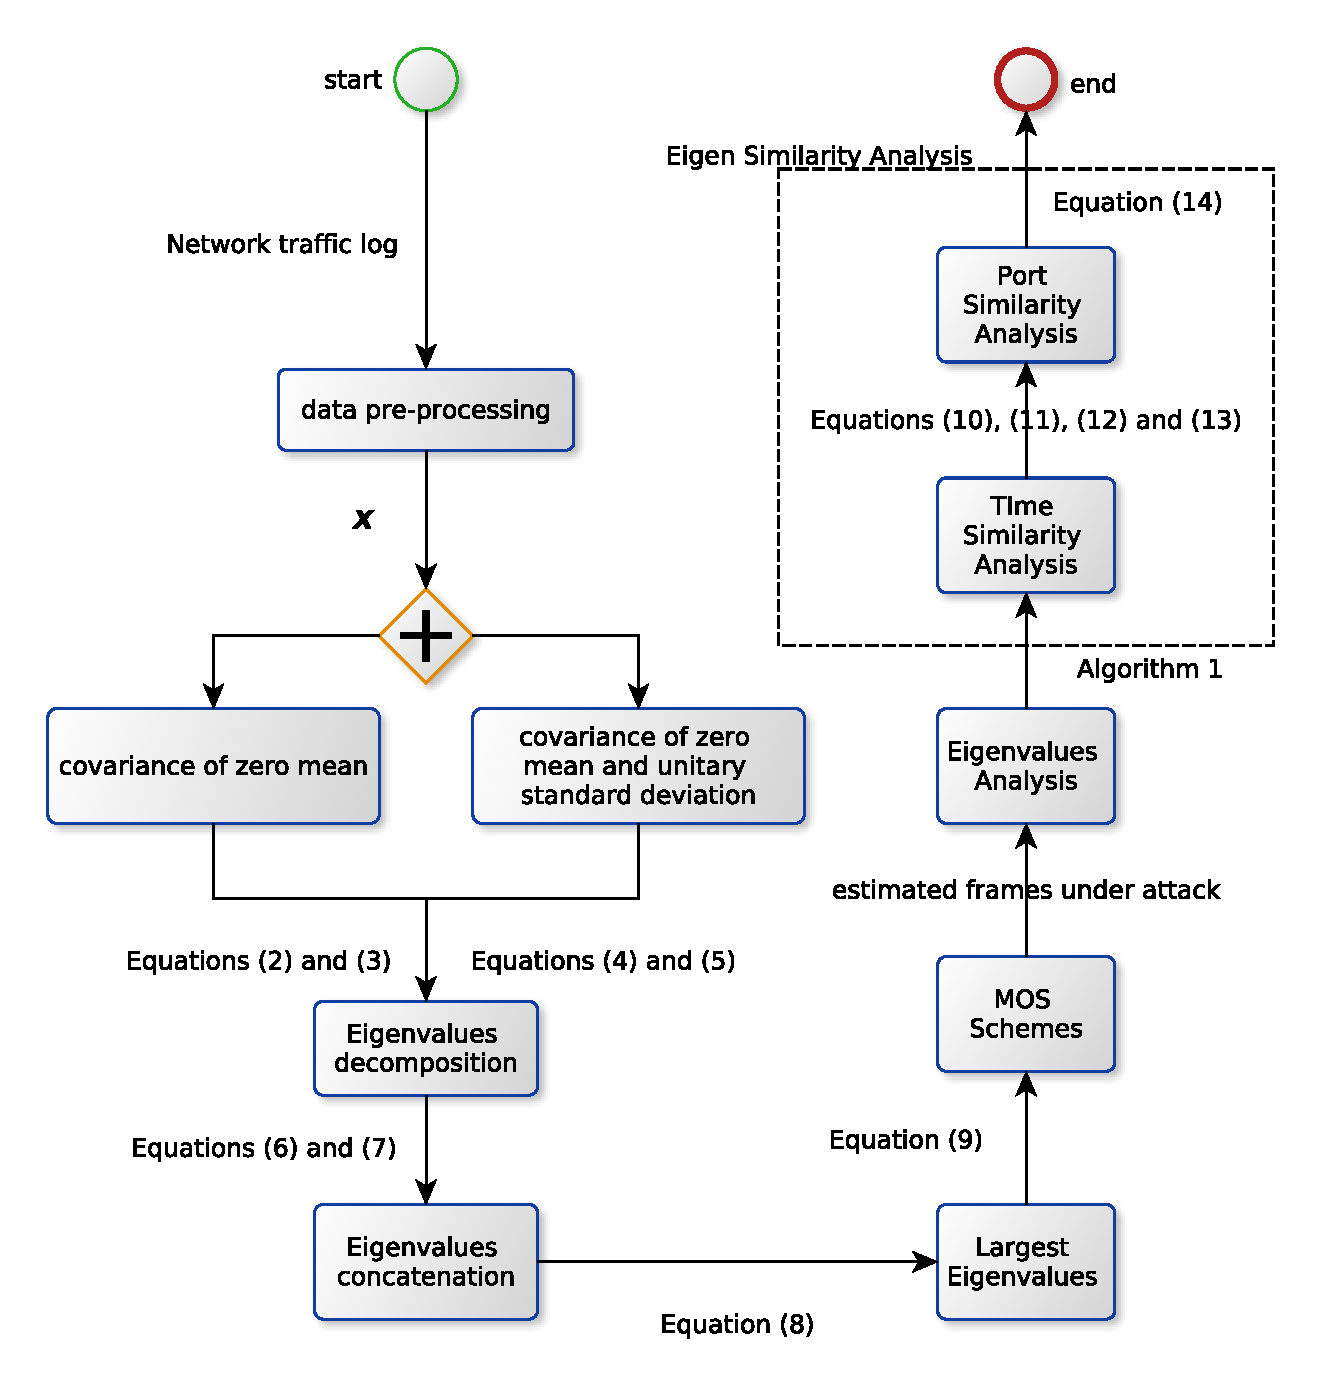
\includegraphics[height=11cm, width=9cm]{results/figures/mos_eigen_similarity.eps}
     \caption{Overview of The Framework for Detection and Identification of Network Attacks.}
     \label{fig:fig80}
\end{figure}

\subsection{Largest Eigenvalue by Time Frames}
\label{sec:prop_LargestEigenvaluebyTimeFrames}

The proposed attack detection algorithm starts by the data pre-processing of a network traffic log containing IP, ports and timestamp of senders and receivers. During this step, the desired information is extracted in order to classify and count packets according to the origin and destination ports, and subsequently this information is grouped by minutes and by time frames.

With the data grouped into $Q$ time frames, the framework considers the time variations of the matrix $\boldsymbol{X}^{(q)} \in \mathbb{R}^{M\times{N}}$, with $q = 1, \ldots, Q$, in order to detect the attack. 

According to flood and port scan attacks' behavior, flood attacks and port scan attacks can be characterized as covariance aware attack \citep{jin2004covariance} and correlation aware attack \citep{lakhina2005mining}, respectively. These characteristics are substantiated by the results obtained through the analysis based on sample covariation of zero mean variables and on covariance of zero mean and unitary standard deviation variables, described in Section \ref{sec:experimentalresults}, which shows that the main components of flood attacks are dominated by the variables with more variance and that the traffic associated with port scan attack does not generate many logs, however, it presents high covariance of zero mean and unitary standard deviation variables.

Therefore, to detect flood attacks, it is necessary to calculate the sample covariance matrix $\boldsymbol{\hat{R}}_{yy}^{(q)}$ of the zero mean samples given by

\begin{equation}\label{eq:eq02}
\boldsymbol{y}_{m}^{(q)} = \boldsymbol{x}_{m}^{(q)} - \bar{\boldsymbol{x}}_{m}^{(q)}.
\end{equation}

The set of obtained vectors $\boldsymbol{y}_{m}^{(q)}$ composes the zero mean matrix $\boldsymbol{Y}^{(q)}$, then the sample covariance matrix $\boldsymbol{\hat{R}}_{yy}^{(q)}$ can be calculated as follows

\begin{equation}\label{eq:eq03}
\boldsymbol{\hat{R}}_{yy}^{(q)} = \frac{1}{N}\boldsymbol{Y}^{(q)}\boldsymbol{Y}^{(q)^{\rm T}}.
\end{equation}

For the detection of the port scan attack, the main components are not dominated by the variables with large variance. Moreover, the portscan traffic presents a highly correlated network traffic. In order to exploit such structure, we compute the sample covariance $\boldsymbol{\hat{R}}_{zz}^{(q)}$ whose variables have zero mean and unitary standard deviation as follows

\begin{equation}\label{eq:eq04}
\boldsymbol{z}_{m}^{(q)} = \frac{\boldsymbol{x}_{m}^{(q)} - \bar{\boldsymbol{x}}_{m}^{(q)}}{\boldsymbol{\sigma}_{m}^{(q)}}.
\end{equation}

The set of vectors $\boldsymbol{z}_{m}^{(q)}$ composes the matrix $\boldsymbol{Z}^{(q)}$, then the sample covariance matrix $\boldsymbol{\hat{R}}_{zz}^{(q)}$ can be calculated via 

\begin{equation}\label{eq:eq05}
\boldsymbol{\hat{R}}_{zz}^{(q)} = \frac{1}{N}\boldsymbol{Z}^{(q)}\boldsymbol{Z}^{(q)^{\rm T}}.
\end{equation}

Once the $\boldsymbol{\hat{R}}_{yy}^{(q)}$ and $\boldsymbol{\hat{R}}_{zz}^{(q)}$ have been obtained for flood and port scan attack detection, respectively, and since the next steps are the same for both sample covariance matrices, we refer to $\boldsymbol{\hat{R}}_{yy}$ and $\boldsymbol{\hat{R}}_{zz}$ as a matrix $\boldsymbol{C}$. Therefore, the following step of the algorithm is the eigenvalue decomposition (EVD), calculated according to (\ref{eq:eq06}), in order to obtain the vector of eigenvalues $\boldsymbol{e}^{(q)}$ associated with each matrix, according to (\ref{eq:eq060}).

\begin{equation}\label{eq:eq06}
\boldsymbol{C}^{(q)} = \boldsymbol{V}^{(q)}\boldsymbol{\Lambda}^{(q)}\boldsymbol{V}^{(q)^{\rm T}},
\end{equation}

\begin{equation}\label{eq:eq060}
\boldsymbol{e}^{(q)} = \rm diag(\boldsymbol{\Lambda}^{(q)}),
\end{equation}

where the operator diag$(\cdot)$ extracts the main diagonal of a matrix.

The eigenvalues should be sorted in descending order, i.e., $\lambda_{1}^{(q)} > \lambda_{2}^{(q)} > \lambda_{3}^{(q)} > ... > \lambda_{m}^{(q)}$. Therefore, the largest eigenvalue of the $q$-th time frame evaluated for the attack detect is given by $\lambda_{1}^{(q)}$.

The concatenation of the eigenvalues vector $\boldsymbol{e}^{(q)}$ for $q = 1, \ldots, Q$ is represented by

\begin{equation}\label{eq:eq07}
\boldsymbol{E} =
\begin{bmatrix}
  \lambda_1^{(1)} & \lambda_1^{(2)} & \lambda_1^{(3)} & \cdots & \lambda_1^{(Q)} \\
  \lambda_2^{(1)} & \lambda_2^{(2)} & \lambda_2^{(3)} & \cdots & \lambda_2^{(Q)} \\
  \lambda_3^{(1)} & \lambda_3^{(2)} & \lambda_3^{(3)} & \cdots & \lambda_3^{(Q)} \\
  \vdots & \vdots & \ddots & \vdots  \\
  \lambda_m^{(1)} & \lambda_m^{(2)} & \lambda_m^{(3)} & \cdots & \lambda_m^{(Q)} \\
\end{bmatrix}.
\end{equation}

Note that since $\lambda_1^{(q)} > \lambda_2^{(q)} > \lambda_3^{(q)} > \cdots > \lambda_{m-1}^{(q)} > \lambda_m^{(q)}$, then the first line of the matrix $\boldsymbol{E}$ contains the largest eigenvalues of each $q$-th time frame, which is the Greatest Eigenvalue Time
Vector (GETV) \cite{tenorio2013greatest}, denoted as 

\begin{equation}\label{eq:eq08}
\boldsymbol{e}_{\rm max} = \boldsymbol{E}\{:,1\} = [ \lambda_1^{(1)}, \lambda_1^{(2)} ... \lambda_1^{(Q)}]
\end{equation}

\subsection{MOS Schemes}
\label{sec:prop_MOSSchemes}

Traditionally the MOS schemes are applied for the eigenvalues of the vector $\boldsymbol{e}^{(q)}$. However, the goal here is to detect the variations of the eigenvalues for different values of $q$. Therefore, instead of using a certain $q$, the proposed approach applies MOS schemes for a vector of the largest eigenvalues of each $q$-th time frame, in order to identify variations and estimate the model order $\hat{d}$, which is the estimated number of time frames under attack. Therefore, $\boldsymbol{e}_{\rm max}$ is sorted in descending order, producing $\sim\boldsymbol{e}_{\rm max}$, that is used as input parameter for MOS schemes, according to $\hat{d} = \rm{MOS}(\sim\boldsymbol{e}_{\rm max})$. Note that some MOS schemes may also require the number of minutes that compose a time frame, as $\hat{d} = \rm{MOS}(\boldsymbol{e}_{\rm max},\emph{Q})$. For more information about MOS, we refer to \ref{sec:mos}.

In our previous work \cite{tenorio2013greatest}, the accuracy of AIC, MDL, EDC, RADOI, EFT and SURE schemes are evaluated for synflood and port scan attack detection, showing that EDC and EFT are effective for detecting this kind of attacks. The present work extends that evaluation to also analyze the effectiveness of the listed MOS schemes for fraggle attack detection, as shown in Section \ref{sec:experimentalresults}.

\subsection{Eigenvalue Analysis}
\label{sec:prop_EigenvalueAnalysis}

After applying the MOS schemes to the vector $\sim\boldsymbol{e}_{\rm max}$, we obtain the estimate of the $\#\boldsymbol{A}$. For instance, in the case of fraggle, synflood and portscan, if $\hat{d} = 1$, , then $\#\boldsymbol{A} = 1$, which means that during the during the $Q$ time frames one attack is present. However, if $\hat{d} = 0$, then $\#\boldsymbol{A} = 0$, and this means that none of these attacks are present. Note that $\hat{d}$ can be greater than 1, indicating the presence of more than one attack.

In Subsection \ref{sec:prop_MOSSchemes}, we obtained only if $\hat{d} = 1$ or $\hat{d} = 0$. However, if $\hat{d} = 1$, the MOS schemes do not provide any information about the $q$-th time frame under attack. The identification of the $q$-th time frame under attack can be carried out through a eigenvalues analysis.

The largest eigenvalue analysis for estimating the $q$-th time frames that are under attack can be expressed according to Algorithm \ref{alg:alg01}, where $\rm{\boldsymbol{\hat{q}}}_{\rm max} \in \mathbb{R}^{\hat{d}}$ denotes a vector of the $q$-th time frames under attack, which is the $q$-th indexes corresponding to the $\hat{d}$ largest eigenvalues of $\boldsymbol{e}_{\rm max}$. Algorithm \ref{alg:alg01} initially identifies the largest value of $\boldsymbol{e}_{\rm max}$, according to Line 2 of Algorithm \ref{alg:alg01}, and its correspondent index, according to Lines 4 and 5 of Algorithm \ref{alg:alg01}. Subsequently, the largest value is removed of $\boldsymbol{e}_{\rm max}$, according to Line 8 of Algorithm \ref{alg:alg01}, and a new iteration is performed until $\boldsymbol{e}_{\rm max} = \{\}$.

\begin{algorithm}[h!]
	\caption{Detection of Time Frames Under Attack}
  	\label{alg:alg01}
	\begin{algorithmic}[1]
		\show\LOOP
	    \ALOOP {$f = 1$ until $f == \hat{d}$} 
	    	    \STATE $q_{\rm value} = \argmax\limits_{\lambda}  \hspace{1 mm} \boldsymbol{e}_{\rm max}$
    	    	    \ALOOP {$i = 1$ until $i == Q$} 
				\IF {$\boldsymbol{e}_{\rm max}^{(i)} == q_{\rm value}$}
				    \STATE $\boldsymbol{\hat{q}}_{\rm max}^{(f)} = i$
				\ENDIF
        		\ENDALOOP
	    		\STATE $\boldsymbol{e}_{\rm max} \rightarrow \boldsymbol{\hat{q}}_{\rm max}^{(f)}$
    		\ENDALOOP
	\end{algorithmic}
\end{algorithm}

After the estimation of the $\rm{\boldsymbol{\hat{q}}}_{\rm max}$ time frames under attack, it is necessary to obtain more details of the detected attacks, such as the $n$-th minutes when the attacks happened and the $m$-th network ports that were attacked. To deal with this problem, the adoption of a similarity analysis between legitimate traffic and the traffic of time frames estimated as under attack is evaluated, analysing the effectiveness of cosine similarity to highlight abnormalies inserted by network traffic attacks. 

\subsection{Eigen Similarity Analysis}
\label{sec:prop_EigenSimilarityAnalysis}

Cosine similarity calculates the cosine of the angle between two vectors, which represents the similarity of values between the selected vectors. Therefore, cosine similarity can be used to evaluate the variation of the most significant eigenvectors of $\boldsymbol{V}^{(q)}$ against the the most significant eigenvectors of time frame detected as under attack, to analyze similarity changes into the most significant eigenvectors caused by the insertion of anomalous traffic \cite{Lee2013}. 

This subsection describes the proposed eigen similarity analysis for detailed attack identification, in complement to the attack estimation carried out through MOS schemes and eigenvalue analysis. In Subsection \ref{sec:prop_TimeSimilarityAnalysis} we present the eigen similarity analysis for identification of time under attack. Next, in Subsection \ref{sec:prop_PortSimilarityAnalysis}, we show how to apply the eigen similarity analysis in order to identify network ports under attack.

\subsubsection{Time Similarity Analysis}
\label{sec:prop_TimeSimilarityAnalysis}

For eigen similarity analyis, we evaluate the cosine similarity in order to identify lacks of similarity between legitimate and malicious traffic, as follows

\begin{equation}\label{eq:eq11}
s_n = \frac{\abs{\boldsymbol{v}^{(q)} \cdot \boldsymbol{v}_{(n)}}}{\norm{\boldsymbol{v}^{(q)}}\norm{\boldsymbol{v}_{(n)}}},
\end{equation}
where $s_n$ denotes the absolute similarity degree of the $n$-th minute, $\boldsymbol{v}^{(q)}$ is the most significant eigenvectors of a selected set of minutes without network attack, and $\boldsymbol{v}_{(n)}$ is the most significant eigenvectors obtained after append the target $n$-th minute of traffic to be performed the flood and port scan attack identification.

The most significant eigenvector $\boldsymbol{v}^{(q)}$, of a time frame $q$ without attack, can be derivated from (\ref{eq:eq06}) and selected according to the eigenvector of the largest eigenvalue $\lambda_1^{(q)}$, which is the principal component of the evaluated matrix. The same calculation shall be performed in order to obtain the target eigenvectors $\boldsymbol{v}_{(n)}$, calculated from a time frame without attack plus minutes of a time frame estimated as under attack, to evaluate the occurrence of network attacks. 

The reference eigenvectors $\boldsymbol{v}^{(q)}$ is calculated from the traffic whithout attack, from a time frame $q$ composed of $Q$ minutes of legitimate network traffic. For the detailed attack identification, each $\boldsymbol{x}^{(\hat{q})}_{(n)}$ vector of each $n$-th minutes of the estimated $\rm{\boldsymbol{\hat{q}}}_{\rm max}$ time frames shall be individually appended into $\boldsymbol{X}^{(q)}$, as represented by

\begin{equation}\label{eq:eq12}
\boldsymbol{X}_{n} = \{\boldsymbol{X}^{(q)} | \boldsymbol{x}^{(\hat{q})}_{(n)}\}.
\end{equation}

The resultant $\boldsymbol{X}_{(n)}$ is necessary to obtain $\boldsymbol{v}_{(n)}$, through (\ref{eq:eq06}), for calculating the similarity degree $s_n$, ranging from 0 to 1, for each $n$-th minute. The $s_n$ denotes the absolute similarity degree of the $n$-th minute in comparison to a well-known traffic without attack, detected through MOS schemes and eigenvalue analysis.

The incremental approach for similarity analysis is based on the incremental appending of network traffic into $\boldsymbol{X}^{(q)}$, where the first evaluation is based on (\ref{eq:eq12}) and the subsequent evaluations is based on (\ref{eq:eq13}), incrementally appending each $n$-th minute until $n=N$.

\begin{equation}\label{eq:eq13}
\boldsymbol{X}_{n} = \{\boldsymbol{X}_{n} | \boldsymbol{x}^{(\hat{q})}_{(n)}\},
\end{equation}

Figure \ref{fig:fig8} ilustrates the network traffic selection for the incremental approach of eigen similarity analysis, where the $\boldsymbol{X}^{(1)}$ is chosen as reference for similarity analysis of the $m$-th minutes of the time frame $q=3$, where one network attack was previously detected. 

\begin{figure}[h!]
     % 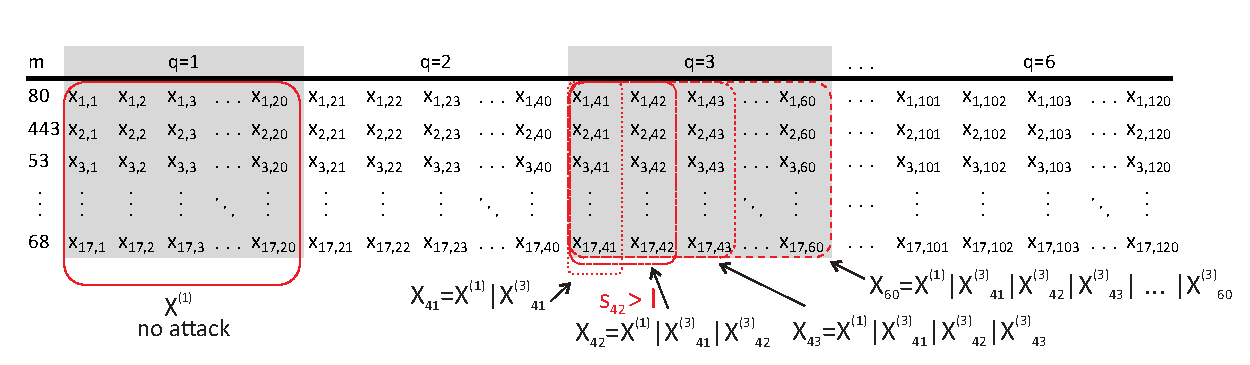
\includegraphics[height=4cm, width=12.4cm]{results/figures/incremental.eps}
     \caption{Traffic selection for incremental approach.}
     \label{fig:fig8}
\end{figure}

The eigen similarity analysis starts at $\boldsymbol{x}^{(3)}_{(41)}$ and is incrementally performed until $\boldsymbol{x}^{(\hat{3})}_{(60)}$, in order to calculate the $s_n$. We assume that $s_n < l$ means an attack identification, according the anomaly on similiarity of $s_n$ to a defined limiar $l$. Therefore, after obtaining the most significant eigenvector $\boldsymbol{v}^{(q)}$ and the target eigenvectors $\boldsymbol{v}_{(n)}$ for eigen similarity analyis, the $s_n$ is calculated according to~(\ref{eq:eq11}).

If $s_n = 1$, then the two eigenvectors are completely similar and no anomaly is detected. Smaller values of $s_n$ mean less similarity and can indicate an anomaly, according to a defined 
threshold $l$, assuming that if $s_n < l$, then a network attack is identified during the $n$-th minute. Therefore, the $s_n$ of each $n$-th minute shall be compared with the threshold $l$ to evaluate if a attack is identified, according to

\begin{equation}\label{eq:eq14}
  \boldsymbol{\hat{n}_{(n)}}=\left\{
  \begin{array}{@{}ll@{}}
    1, & \text{if}\ s_n < l \\
    0, & \text{otherwise}
  \end{array}\right.
\end{equation}
where $\boldsymbol{\hat{n}}_{(n)}$ denotes a vector of $n$-th minutes detected as under attack.

The eigen similarity analysis can also be applied in an individual fashion, where each $n$-th minute must be individually appended into $\boldsymbol{X}^{(q)}$, as shown by Figure \ref{fig:fig9}.

\begin{figure}[h!]
     % 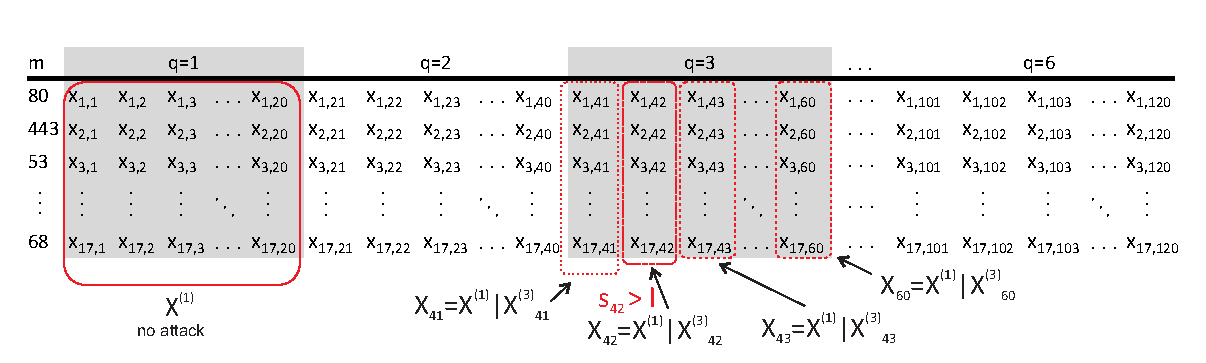
\includegraphics[height=4cm, width=12.4cm]{results/figures/individualized.eps}
     \caption{Traffic selection for individual approach.}
     \label{fig:fig9}
\end{figure}

The incremental and the individual approaches can be combined to obtain the incremental individualized approach, where each minute is incrementally appended into the selected $\boldsymbol{X}^{(q)}$ for obtaining $\boldsymbol{v}_{(n)}$ to similarity analysis of the $n$-th minute, until detect the first $n$-th minute under attack. Subsequently, $\boldsymbol{X}_n$ becomes the new reference of traffic without network attack and each subsequent minute must have its similarity individually evaluated, as shown in Figure \ref{fig:fig2}.

\begin{figure}[h!]
     % 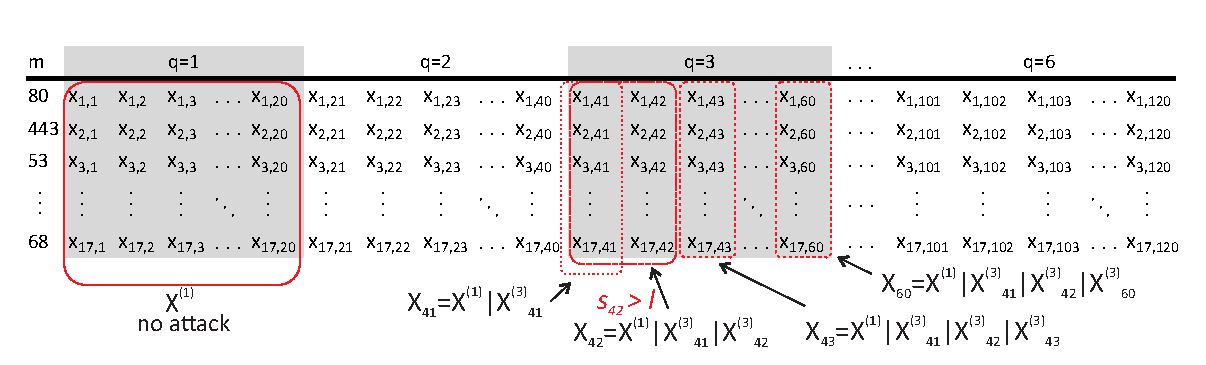
\includegraphics[height=4cm, width=12.4cm]{results/figures/incremental_individualized.eps}
     \caption{Traffic selection for incremental individualized approach.}
     \label{fig:fig2}
\end{figure}

This approach of incremental similarity analysis followed by individual analysis after an attack detection allows to identify the attack period, highlighting the first and last time under attack. This identification is possible due to the variation of the most significant eigenvectors, which becomes more significant when compared a traffic under attack against a traffic with no attack, according to results which are discussed in Section \ref{sec:experimentalresults}.

\subsubsection{Port Similarity Analysis}
\label{sec:prop_PortSimilarityAnalysis}

Given $\boldsymbol{\hat{n}}$, which is the set of $n$-th minutes under attack, it is still necessary to obtain more details about the identified network attack, such as the network ports that are attacked during each $n$-th minute identified as under attack. Hence, it is also applied the cosine similarity analysis to identify variation of the most significant eigenvectors, caused by the insertion of anomalous network traffic by a selected $m$-th port during a $n$-th minute. 

For detection of ports under attack, the $\boldsymbol{v}^{(q)}$ last most significant eigenvectors without attack shall be used as reference for similarity analysis against the $\boldsymbol{v}_{(n)}$ identified as under attack, individually evaluating the cosine similarity of each $m$-th port of all $\boldsymbol{\hat{n}}$ minutes.

Therefore, $\boldsymbol{v}^{(q)}$ should be calculated from the last $\boldsymbol{X}^{(q)}$ time frame without attack, and $\boldsymbol{v}_{(m,\hat{n})}$ should be calculated from the same traffic appened of all $n$-th minutes until the identified minute under attack, denoted as $\boldsymbol{X}_n$. 

For similarity analyis, each $m$-th port of the last $n$-th minute of $\boldsymbol{X}_n$, denoted as $x_{(m,n)}$, shall be individually replaced by the traffic of the evaluated $m$-th port of the $\hat{n}$-th minute under attack, denoted as $x^{(\hat{q})}_{(m,\hat{n})}$, in order to identify significant variation on similarity caused by the traffic of the $m$-th port. 

This approach for detection of ports under attack via similarity analysis is given by

\begin{equation}\label{eq:eq15}
  \left\{
  \begin{array}{@{}ll@{}}
    x_{(m,n)} = x^{(\hat{q})}_{(m,\hat{n})} \\
    \\
    s_{m,\hat{n}} = \frac{\abs{\boldsymbol{v}^{(q)} \cdot \boldsymbol{v}_{(m,\hat{n})}}}{\norm{\boldsymbol{v}^{(q)}}\norm{\boldsymbol{v}_{(m,\hat{n})}}},
  \end{array}\right.
\end{equation}

where $x^{(\hat{q})}_{(m,\hat{n})}$ denotes the $m$-th port of the selected $n$-th minute identified as under attack and $x_{(m,n)}$ denotes the $m$-th port of the last $n$-th minute of $\boldsymbol{X}_n$, which is used to calculate the $\boldsymbol{v}_{(m,\hat{n})}$ most significant eigenvectors that contains the traffic of the $m$-th port of the $\hat{n}$-th minute identified as under attack.

Once $\boldsymbol{v}^{(q)}$ and $\boldsymbol{v}_{(m,\hat{n})}$ are obtained, then the $s_{m,\hat{n}}$ similarity degree can be calculated in order to identify if the traffic replacement highlights the adition of anomalous traffic by the evaluated $m$-th port during the $\hat{n}$-th minute previously identified as under attack. 

This procedure should be repeated for each $m$-th target port of $\boldsymbol{\hat{n}}$, in order to individually identify the network ports under attack during each $\hat{q}$-th time frame.

%%%%%%%%%%%%%%%%%%%%%%%%%%%%%%%%%%%%%%%%%%%%%%%%%%%%%%%%%%%%%%%%%%%%%%%%%%%%%%%%%%%%%%%%%%%%%%%%%%%%%%%%%%%%%%%%%%%%%%%%%%%%%%%%%%%%%%%%%%%%%%%%%%%%%%%%%%%%%%%%%%%%%%%%%%%%%%%%%%%%%%%%%%%%%%%%%%%%%%%%%%%%%%%%%%%%%%%%%%%%
\section{Experiments and Results}
\label{sec:experimentalresults}

This section presents the performed experiments and the acquired results. First, in Section \ref{sec:AnalyzedScenario}, the experimental scenario adopted in the experiments is summarized. Then, Section \ref{sec:largesteigenvaluesanalysis} shows the results of the largest eigenvalue analysis by time frames for the experimental scenario. In Section \ref{sec:MOSSchemesEvaluation} are described the results of the evaluated MOS schemes for attack detection in the simulated dataset. Section \ref{sec:EigenvalueAnalysis} presents the results of the eigenvalue analysis for identification of time frames under attack, Section \ref{sec:EigenSimilarityAnalysis} shows the results of similarity analysis for detailed flood and port scan identification for the experimental scenario. Section \ref{sec:DarpaEvaluation} presents the results of the largest eigenvalue analysis, model order selection and the eigenvalue analysis for flood and probe attack detection in the DARPA 1998 dataset.

\subsection{Experimental Scenario}
\label{sec:AnalyzedScenario}

The experiment time is 120 minutes, separated into six time frames, with each time frame corresponding to twenty minutes. Therefore, as the time of each sampling period is one minute, then $N = 20$. For each time frame $q$, a traffic matrix $\boldsymbol{X}^{(q)} \in \mathbb{R}^{17 \times 20}$ was obtained, as well as a covariance $\boldsymbol{\hat{R}}_{yy}^{(q)} \in \mathbb{R}^{17 \times 17}$ (calculated via (\ref{eq:eq03})) and a sample covariance matrix $\boldsymbol{\hat{R}}_{zz}^{(q)} \in \mathbb{R}^{17x17}$, assuming that $q = 1, 2, 3, 4, 5$ and $6$. 

The simulation started at 21:00h, the first time frame was from 21:00h until 21:20h ($q = 1$), the second was from 21:20h until 21:40h ($q = 2$), the third was from 21:40h to 22:00h ($q = 3$), the fourth was from 22:00h until 22:20h ($q = 4$), the fifth was from 22:20h until 22:40h ($q = 5$), and finally, the sixth was from 22:40h until 23.00h ($q = 6$). During the simulation, the victim made legitimate access, and the attacker performed the following attacks: at 21:54h ($q = 3$) was performed a port scan, at the interval ranging from 22:10h to 22:20h ($q = 4$) a synflood attack was simulated, and at the interval from 22:30h to 22:40h ($q = 5$) a fraggle attack was performed.

\subsection{Largest Eigenvalues Analysis}
\label{sec:largesteigenvaluesanalysis}

For the evaluation of MOS Schemes accuracy for flood and port scan detection, the framework defines that it is necessary to obtain the largest eigenvalue of each time frame, through eigen decomposition from a covariance of zero mean variables or covariance matrix of zero mean and unitary standard deviation variables, calculated from the evaluated traffic, as described in Section \ref{sec:prop_getv}. Through eigenvalue analysis of traffic with flood or port scan attacks, it is possible to visualize a significant difference between the largest eigenvalues and the remain eigenvalues, which can indicate a relationship between an outlier and time frames under attack.

\begin{figure}[h!]
	\centering
     % \includegraphics[height=6cm, width=8cm]{results/figures/eigenvalues_synflood.eps} 
     \caption{Eigenvalues of the sample covariance matrix (synflood).}
     \label{fig:fig10}
\end{figure}

Figure \ref{fig:fig10} depicts the eigenvalues calculated from sample covariance matrix of the network traffic used to evaluate the synflood attack identification. In Figure \ref{fig:fig10}, the largest eigenvalue related to the simulated synflood attack ($q = 4$) stands out significantly from the other eigenvalues.

Figure \ref{fig:fig11} illustrates the eigenvalues calculated from sample covariance matrix of the matrix used for fraggle attack detection. In Figure \ref{fig:fig10}, the largest eigenvalue related to the simulated synflood attack ($q = 5$) stands out significantly from the other eigenvalues, in accordance with the result shown in Figure \ref{fig:fig10} for the synflood attack analysis.

\begin{figure}[h!]
	\centering
     % \includegraphics[height=6cm, width=8cm]{results/figures/eigenvalues_fraggle.eps}
     \caption{Eigenvalues of the sample covariance matrix (fraggle).}
     \label{fig:fig11}
\end{figure}

Figure \ref{fig:fig12} depicts the eigenvalues calculated from covariance matrix of zero mean and unitary standard deviation variables, of the network traffic matrix evaluated for port scan detection. 

\begin{figure}[h!]
	\centering
     % \includegraphics[height=6cm, width=8cm]{results/figures/eigenvalues_portscan.eps}
     \caption{Eigenvalues of the covariance matrix of zero mean and unitary standard deviation (port scan).}
     \label{fig:fig12}
\end{figure}

As analyzed for the synflood and fraggle attacks, note that the largest eigenvalue, related to this attack ($q = 3$), stands out significantly from the others eigenvalues.

Table \ref{tab:tab3} presents the values of the largest eigenvalues of each time frame $q$-th for port scan, synflood and fraggle detection. 

\begin{table}[h!]
  \centering
  \footnotesize
  \caption{Largest Eigenvalue related to attacks detection}
  \label{tab:tab3}
  \begin{tabular}{ c c c c c }
	\toprule
	\multirow{3}{*}{\textbf{Time Frame} $q$} &\multicolumn{4}{c }{\textbf{Vectors GETV}}\\ 
			\hhline{~----}
		&\textbf{Detection of}	 &\textbf{Detection of}	 &\textbf{Detection of}	 &\textbf{Detection of}\\
		&\textbf{\emph{synflood/fraggle}}	 &\textbf{\emph{synflood}}	 &\textbf{\emph{fraggle}}	 &\textbf{\emph{port scan}}\\
	\midrule
	1 &1887545 &1887545 &1887545 &2,0734 \\
	2 &2341327 &2341327 &2341327 &2,1451 \\
	3 &3213867 &3213867 &3213867 &10,0718 \\
	4 &133238294 &133238294 &731229 &2,1620 \\
	5 &92384021611 &6367983 &92384021611 &2,4253 \\
	6 &708335 &708335 &708335 &1,7948 \\
    \bottomrule
  \end{tabular}
\end{table}

In Table \ref{tab:tab3}, note the significant variation of the eigenvalues associated with attacks, in comparison to the others. At $q = 4$, where the synflood attack occurred, the maximum eigenvalue obtained is approximately 21 times larger than the second one. At $q = 5$, where the fraggle attack occurred, the maximum eigenvalue obtained is about 29,000 times larger than the second one. At $q = 3$, where the port scan attack occurred, the maximum eigenvalue obtained is approximately 4 times larger than the second one. In the last case, for port scan attack detection, although the largest eigenvalue presented no too large variance to the second one, if compared to synflood or fraggle attacks, it clearly deviates from the remaining largest eigenvalues.

These results highlight that all $q$-th time frames where a network attack was simulated, present high significant variance between the largest eigenvalue and the remaining eigenvalues, obtained from sample covariance matrix, for flood detection, or from covariance matrix of zero mean and unitary standard deviation variables, for port scan detection. Therefore, we propose to apply the vector of the largest eigenvalues to MOS schemes in order to evaluate their accuracy for identification of time frames under attack, motivated by the fact that it is relevant to apply MOS schemes to automate the attack detection process, taking into account the characteristics of the evaluated eigenvalues.

\subsection{MOS Schemes Evaluation}
\label{sec:MOSSchemesEvaluation}

In \cite{tenorio2013greatest}, we evaluate the accuracy of AIC, MDL, EDC, RADOI, EFT and SURE MOS schemes \cite{da2009comparison,tenorio2013greatest} for synflood and port scan attack detection. In this work we extend that evaluation for fraggle attack detection, applying the same schemes to fraggle attack detection over the traffic presented in Section \ref{sec:datamodel}, as results shown in Table \ref{tab:tab4}.

\begin{table}[h!]
  \centering
  \scriptsize
  \caption{MOS schemes applied to port scan and flood detection}
  \label{tab:tab4}
  \begin{tabular}{ c c c c c c c c }
	\toprule
	\multirow{2}{*}{\textbf{Type of analysis} $q$} &\multicolumn{6}{c}{\textbf{MOS schemes (estimated model order $\hat{d}$)}} &{\textbf{(d)}}\\ 
			\hhline{~------~}
		&\textbf{AIC} &\textbf{MDL} &\textbf{EDC} &\textbf{RADOI} &\textbf{EFT} &\textbf{SURE}\\
	\midrule
	Detection of synflood \\(presence of attack) &2 &1 &\textbf{1} &5 &\textbf{1} &4 &\textbf{1} \\
	Detection of synflood \\(absence of attack) &1 &1 &\textbf{0} &1 &\textbf{0} &3 &\textbf{0} \\
	\midrule
	Detection of fraggle \\(presence of attack) &1 &1 &\textbf{1} &5 &\textbf{1} &4 &\textbf{1} \\
	Detection of fraggle \\(absence of attack) &1 &1 &\textbf{0} &1 &\textbf{0} &3 &\textbf{0} \\
	\midrule
	Detection of port scan \\(presence of attack) &1 &1 &\textbf{1} &1 &\textbf{1} &9 &\textbf{1} \\
	Detection of port scan \\(absence of attack) &0 &0 &\textbf{0} &1 &\textbf{0} &1 &\textbf{0} \\
	\midrule
	Detection of synflood/fraggle \\(presence of attack) &2 &2 &\textbf{2} &5 &\textbf{2} &5 &\textbf{2} \\
	Detection of synflood/fraggle \\(absence of attack) &1 &1 &\textbf{0} &1 &\textbf{0} &3 &\textbf{0} \\
    \bottomrule
  \end{tabular}
\end{table}

Note that $\hat{d} = 1$, if there is attack, while $\hat{d} > 1$ indicates more than one attack. An example of this could be seen for attack detection via EFT for traffic containing synflood and fraggle attacks, showing $\hat{d} = 2$, which indicates the presence of two attacks, as expected by the $d$ real values of Table \ref{tab:tab4}. 

In Table \ref{tab:tab4}, two MOS schemes outperforms from the others, EDC and EFT. Efficient Detection Criterion (EDC) and Exponential Fitting Test (EFT) are the most effective schemes, correctly estimating the number of attacks in comparison to the expected values for effetctive attack detection, as defined by the column of real values in Table \ref{tab:tab4}. The AIC and MDL schemes are satisfactory only for port scan detection, however SURE and RADOI schemes did not show effective results for port scan or flood detection.

Although EDC and EFT presented the same accuracy on the evaluation, the EDC scheme requires less processing time than EFT, which is an important criteria to select EDC as the MOS scheme for flood and port scan detection on the remain experiments.

According to Table \ref{tab:tab4}, EDC and EFT estimated correctly the number of attacks of a time frame vector, indicating that ocurred $\hat{d}$ network attacks, but not providing additional details, what highlights the necessity of complementary approaches in order to estimate the time and ports under attack. Hence, we propose apply eigen analysis to estimate the $q$-th time frames under attack and eigen similarity analysis to estimate the minutes and ports under attack.

\subsection{Eigenvalue Analysis}
\label{sec:EigenvalueAnalysis}

According to the results presented in Section \ref{sec:largesteigenvaluesanalysis}, the largest eigenvalue stands out significantly from the others eigenvalues of an evaluated $q$-th time frame. This behavior can also be observed in the largest eigenvalues analysis, according to results presented in Table \ref{tab:tab3}, where it is possible to observe that the $\hat{d}$ largest eigen values of the time frames under attacks stand out significantly from the others largest eigenvalues. 

Therefore, we conclude that the $\hat{d}$ largest eigenvalues correspond to the respectives $q$-th time frames under attack, which is denoted by $\rm{\boldsymbol{\hat{q}}}_{\rm max}$ and can be calculated according to Algorithm \ref{alg:alg01}.

\subsection{Eigen Similarity Analysis}
\label{sec:EigenSimilarityAnalysis}

This paper proposes applying eigen similarity analysis to detect time and ports under attack, from each $q$-th time frames under attack defined by $\rm{\boldsymbol{\hat{q}}}_{\rm max}$. Hence, the proposed framework is applied to the time frames where $q=3$, $q=4$ and $q=5$ to respectively evaluate its effectiveness for port scan, synflood and fraggle attack detection.

\subsubsection{Time Analysis}
\label{sec:TimeAnalysis}

Three approaches were evaluated for eigen similarity analysis: incremental, individual and incremental individualized approaches. For the incremental individualized approach, each minute is incrementally appended into the selected $\boldsymbol{X}^{(q)}$ for obtaining $\boldsymbol{v}_{(n)}$ to similarity analysis of the $n$-th minute, until detect the first $n$-th minute under attack. Subsequently, $\boldsymbol{X}_n$ became the new reference of traffic without network attack and each subsequent minute must have its similarity individually evaluated. For the incremental approach, each $n$-th minute must be incrementally appended into $\boldsymbol{X}^{(q)}$, for obtaining the next eigenvectors $\boldsymbol{v}_{(n)}$ for individual time similarity analyis. For the individual approach, each $n$-th minute must be individually appended into $\boldsymbol{X}^{(q)}$, without incremental append, but doing individual appended into $\boldsymbol{X}^{(q)}$ for obtaining the next eigenvectors $\boldsymbol{v}_{(n)}$ for individual similarity analyis.

Table \ref{tab:tab5} presents the results of the evaluation of three approaches for similarity analysis of eigenvectors for port scan detection.

\begin{table}[h!]
  \centering
  \footnotesize
  \caption{Eigen Similarity Analysis for Port Scan Detection}
  \label{tab:tab5}
  \begin{tabular}{ c c c c c c }
	\toprule
	\multirow{2}{*}{\textbf{Time Frame} $q$} &\multirow{2}{*}{\textbf{Time} $n$}   &\multicolumn{3}{c}{\textbf{Similarity Analysis}} &\multirow{2}{*}{\textbf{Attack?}}\\ 
			\hhline{~~---~}
			& &\textbf{Incremental Individualized} &\textbf{Incremental} &\textbf{Individual}\\
	\midrule
	3 &1 &0.9946 &0.9946 &0.9946 &no \\
	3 &2 &0.9934 &0.9934 &0.9999 &no \\
	3 &3 &0.9912 &0.9912 &0.9999 &no \\
	3 &4 &0.9888 &0.9888 &0.9999 &no \\
	3 &5 &0.9856 &0.9856 &0.9998 &no \\
	3 &6 &0.9840 &0.9840 &0.9999 &no \\
	3 &7 &0.9824 &0.9824 &1.0000 &no \\
	3 &8 &0.9794 &0.9794 &0.9999 &no \\
	3 &9 &0.9673 &0.9673 &0.9926 &no \\
	3 &10 &0.9674 &0.9674 &0.9997 &no \\
	3 &11 &0.9733 &0.9733 &0.9993 &no \\
	3 &12 &0.9702 &0.9702 &0.9993 &no \\
	3 &13 &0.9677 &0.9677 &0.9999 &no \\
	3 &14 &0.9646 &0.9646 &0.9998 &no \\
	3 &15 &0.0216 &0.0216 &0.0276 &yes \\
	3 &16 &0.9621 &0.0209 &1.0000 &no \\
	3 &17 &0.9611 &0.0199 &0.9998 &no \\
	3 &18 &0.9612 &0.0191 &0.9999 &no \\
	3 &19 &0.9613 &0.0186 &0.9998 &no \\
	3 &20 &0.9638 &0.0190 &1.0000 &no \\
    \bottomrule
  \end{tabular}
\end{table}

Table \ref{tab:tab5} shows the evaluation of the time frame $q=3$, when the port scan attack was simulated, considering the incremental individualized, incremental and individual approaches for eigen similarity analysis. According to the presented results, it is possible to observe the high similarity between network traffic without attack, which was larger than 0.9610 for all evaluated cases, and emphasize the expressive low similarity when evaluated the traffic with the simulated port scan attack ($n=15$), which was lower than 0.0276 for all evaluated approaches.

Comparing the approaches for similarity analysis, it is possible to observe that all approaches highlight the low similarity when evaluated the traffic under attack. However, the incremental approach figured out low similarity for times without attack, where $n=16, 17, 18, 19, 20$, what indicates that the incremental approach can produce false posive results. This behavior occurs because the incremental approaches appends all selected traffic into the reference traffic for comparison against the original reference traffic, what makes more evident the first lack of similarity but reduces the changing detection capability after an attack detection.

Table \ref{tab:tab6} presents the results of the evaluation of the similarity analysis of eigenvectors for synflood detection. It shows the evaluation of the time frame $q=4$, when the synflood attack is simulated, considering the incremental individualized, incremental and individual approaches for eigen similarity analysis. According to the results, it is possible to observe the high similarity between network traffic without attack, which is larger than 0.9907 for all evaluated cases, and emphasize the expressive low similarity when evaluated the traffic with synflood attack (between $n=11$ and $n=20$), which is lower than 0.1244 for all evaluated approaches.

\begin{table}[h!]
  \centering
  \footnotesize
  \caption{Eigen Similarity Analysis for Synflood Detection}
  \label{tab:tab6}
  \begin{tabular}{ c c c c c c }
	\toprule
	\multirow{2}{*}{\textbf{Time Frame} $q$} &\multirow{2}{*}{\textbf{Time} $n$}   &\multicolumn{3}{c}{\textbf{Similarity Analysis}} &\multirow{2}{*}{\textbf{Attack?}}\\ 
			\hhline{~~---~}
			& &\textbf{Incremental Individualized} &\textbf{Incremental} &\textbf{Individual}\\
	\midrule
	4 &1 &1.0000 &1.0000 &1.0000 &no \\
	4 &2 &0.9999 &0.9999 &1.0000 &no \\
	4 &3 &0.9997 &0.9997 &0.9999 &no \\
	4 &4 &0.9998 &0.9998 &1.0000 &no \\
	4 &5 &0.9965 &0.9965 &0.9908 &no \\
	4 &6 &0.9975 &0.9975 &1.0000 &no \\
	4 &7 &0.9977 &0.9977 &1.0000 &no \\
	4 &8 &0.9980 &0.9980 &1.0000 &no \\
	4 &9 &0.9987 &0.9987 &0.9999 &no \\
	4 &10 &0.9991 &0.9991 &1.0000 &no \\
	4 &11 &0.0085 &0.0085 &0.0284 &yes \\
	4 &12 &0.0162 &0.0120 &0.0343 &yes \\
	4 &13 &0.0248 &0.0158 &0.0427 &yes \\
	4 &14 &0.1243 &0.0185 &0.1041 &yes \\
	4 &15 &0.0082 &0.0162 &0.0103 &yes \\
	4 &16 &0.0404 &0.0070 &0.0580 &yes \\
	4 &17 &0.0397 &0.0007 &0.0573 &yes \\
	4 &18 &0.0408 &0.0042 &0.0584 &yes \\
	4 &19 &0.0408 &0.0079 &0.0584 &yes \\
	4 &20 &0.0477 &0.0092 &0.0757 &yes \\
    \bottomrule
  \end{tabular}
\end{table}

The incremental approach produces better results if compared with other evaluated approaches, with lower values and maximum of 0.0185 for times under attack, but this approach presents change detection limitation after the first outlier of similarity, as shown in Table \ref{tab:tab5} for port scan detection. 

Comparing the incremental individualized and the individual approaches for eigen similarity analysis, it is possible to observe that the incremental individualized approach obtain lowest values for almost all cases, except for the time $n=14$, where incremental individualized approach identified a larger similarity than the individual approach. The incremental individualized appends information about each evaluated traffic, therefore it incorporates traffic behaviors that can reduce the outlier capability detection, as ocurred for the time $n=14$.

Table \ref{tab:tab7} presents the results of the eigen similarity analysis evaluation for fraggle detection.

\begin{table}[h!]
  \centering
  \footnotesize
  \caption{Eigen Similarity Analysis for Fraggle Detection}
  \label{tab:tab7}
  \begin{tabular}{ c c c c c c }
	\toprule
	\multirow{2}{*}{\textbf{Time Frame} $q$} &\multirow{2}{*}{\textbf{Time} $n$}   &\multicolumn{3}{c}{\textbf{Similarity Analysis}} &\multirow{2}{*}{\textbf{Attack?}}\\ 
			\hhline{~~---~}
			& &\textbf{Incremental Individualized} &\textbf{Incremental} &\textbf{Individual}\\
	\midrule
	5 &1 &1.0000 &1.0000 &1.0000 &no \\
	5 &2 &0.9999 &0.9999 &1.0000 &no \\
	5 &3 &1.0000 &1.0000 &1.0000 &no \\
	5 &4 &0.9999 &0.9999 &1.0000 &no \\
	5 &5 &0.9993 &0.9993 &0.9997 &no \\
	5 &6 &0.9993 &0.9993 &0.9997 &no \\
	5 &7 &0.9994 &0.9994 &1.0000 &no \\
	5 &8 &0.9995 &0.9995 &1.0000 &no \\
	5 &9 &0.9995 &0.9995 &1.0000 &no \\
	5 &10 &0.9995 &0.9995 &1.0000 &no \\
	5 &11 &0.0031 &0.0031 &0.0021 &yes \\
	5 &12 &0.0019 &0.0025 &0.0009 &yes \\
	5 &13 &0.0030 &0.0026 &0.0020 &yes \\
	5 &14 &0.0030 &0.0027 &0.0020 &yes \\
	5 &15 &0.0030 &0.0028 &0.0020 &yes \\
	5 &16 &0.0012 &0.0025 &0.0002 &yes \\
	5 &17 &0.0030 &0.0026 &0.0020 &yes \\
	5 &18 &0.0030 &0.0026 &0.0020 &yes \\
	5 &19 &0.0030 &0.0027 &0.0020 &yes \\
	5 &20 &0.0069 &0.0023 &0.0083 &yes \\
    \bottomrule
  \end{tabular}
\end{table}

For fraggle attack detection, the lack of similarity between legitimate and malicious traffic was more evident than for the evaluation of synflood and port scan detecion. This behavior can be explained by the number of packets generated through the fraggle attack simulation, that was significative larger than the number of packets generated during the synflood simulation. Considering the three approaches, the largest value for times under attack was 0.0083, while the shortest value for times without attacks was 0.9993. 

Therefore, considering the evaluation for port scan, synflood and fraggle detection, the incremental approach can produce false positive results, while the individual and incremental individualized approaches produce quite similar results, even though the individual approach be more simple and require less memory and processing time.

These results highlight the capability of change detection based on similarity between legitimate and malicious traffic from flood or port scan attacks, endorsing the effectiveness and safety for adoption of threshold for attack detection through eigen similarity analysis.

\subsubsection{Port Analysis}
\label{sec:PortAnalysis}

Given $\hat{N}$, which is the set of estimated $n$-th minutes under attack, it is possible to apply cosine similarity analysis to identify variation of the most significant eigenvectors, caused by the insertion of anomalous network traffic by a selected $m$-th port, during a $n$-th minute. Therefore, the incremental individualized and individual approaches of eigen similarity analysis were evaluated, for detection of ports under flood and port scan attacks, according to results presented in following tables. For this evaluation, the $v$ last most significant eigenvectors without attack was used as reference for similarity analysis against each target port $m$-th.

Table \ref{tab:tab8} presents the results of the evaluation of eigen similarity analysis for detection of ports under port scan attack, showing only the time frame $q=3$ and minute $n=15$, due to the simulated port scan attack occurred only at this time, although the remain time frame has been completely evaluated and presented high similarity to the reference of traffic without network attack.

\begin{table}[h!]
  \centering
  \footnotesize
  \caption{Eigen Similarity Analysis for Detection of Ports Under Port Scan Attack (q=3 and n=15)}
  \label{tab:tab8}
  \begin{tabular}{ c c c c }
	\toprule
	\multirow{2}{*}{\textbf{Port} $p$}   &\multicolumn{2}{c}{\textbf{Approaches}} &\multirow{2}{*}{\textbf{Attack?}}\\ 
			\hhline{~--~}
			&\textbf{Incremental Individualized} &\textbf{Individual}\\
	\midrule
	80 &0.9999 &0.9999 &no \\
	443 &0.9999 &0.9999 &no \\
	53 &0.9999 &0.9999 &no \\
	21 &0.9999 &0.9997 &yes \\
	22 &0.0298 &0.9997 &yes \\
	23 &0.0298 &0.9997 &yes \\
	25 &0.0298 &0.9997 &yes \\
	110 &0.0298 &0.9997 &yes \\
	143 &0.0298 &0.9997 &yes \\
	161 &0.0298 &0.9997 &yes \\
	69 &0.0298 &0.9997 &yes \\
	123 &0.0298 &0.9997 &yes \\
	445 &0.0298 &0.9997 &yes \\
	600 &0.9999 &0.9999 &no \\
	19 &0.9999 &0.9999 &no \\
	67 &0.9999 &0.9999 &no \\
	68 &0.9999 &0.9999 &no \\
    \bottomrule
  \end{tabular}
\end{table}

The incremental individualized approach presented more sensibility to anomaly detection than the individual approach, the former produced the identification of a low similarity of 0.0298 for almost all ports under attack, unless the port 21, although the simulation has attacked this port. The individual approach was not able to identify low similarity for ports under attack, resunting in values of 0.9997 for ports with anomalous traffic and 0.9999 for ports without network attack.

For the evaluation of the proposed approaches for identification of ports under synflood and fraggle attack, all minutes of each time frame, in which one attack location was estimated, were analyzed. Even though, due to space limitations, only the results of the firt minute where a low similarity was idenfified will be shown such as where $n=11$. Nevertheless, the results obtained for the evaluation of traffic without attack presented high similarity to the reference traffic, with similarities close to 0.9999, and the evaluation of the other minutes under attack presented results quite similar to the resuts shown in the Tables \ref{tab:tab9} and \ref{tab:tab10}.

Table \ref{tab:tab9} presents the results of the evaluation of eigen similarity analysis for detection of ports under synflood attack, showing only the time frame $q=4$ and minute $n=11$.

\begin{table}[h!]
  \centering
  \footnotesize
  \caption{Eigen Similarity Analysis for Detection of Ports Under Synflood Attack (q=4 and n=11)}
  \label{tab:tab9}
  \begin{tabular}{ c c c c }
	\toprule
	\multirow{2}{*}{\textbf{Port} $p$}   &\multicolumn{2}{c}{\textbf{Approaches}} &\multirow{2}{*}{\textbf{Attack?}}\\ 
			\hhline{~--~}
			&\textbf{Incremental Individualized} &\textbf{Individual}\\
	\midrule
	80 &1.0000 &1.0000 &no \\
	443 &1.0000 &1.0000 &no \\
	53 &1.0000 &1.0000 &no \\
	21 &1.0000 &1.0000 &nos \\
	22 &1.0000 &1.0000 &no \\
	23 &1.0000 &1.0000 &no \\
	25 &1.0000 &1.0000 &no \\
	110 &1.0000 &1.0000 &no \\
	143 &1.0000 &1.0000 &no \\
	161 &1.0000 &1.0000 &no \\
	69 &1.0000 &1.0000 &no \\
	123 &1.0000 &1.0000 &no \\
	445 &1.0000 &1.0000 &no \\
	600 &0.0077 &0.0427 &yes \\
	19 &1.0000 &1.0000 &no \\
	67 &1.0000 &1.0000 &no \\
	68 &1.0000 &1.0000 &no \\
    \bottomrule
  \end{tabular}
\end{table}

According to results presented in Table \ref{tab:tab9}, both approches identifies low similarity for the traffic of port 600, which is the target port of the simulated synflood attack, but the incremental individualized approach identifies the lowest similarity and presents better sensibility to identification of synflood attack through eigen similarity analysis assisted by threshold definition.

Table \ref{tab:tab10} presents the results of the evaluation of eigen similarity analysis for detection of ports under fraggle attack, showing only the time frame $q=5$ and minute $n=11$.

\begin{table}[h!]
  \centering
  \footnotesize
  \caption{Eigen Similarity Analysis for Detection of Ports Under Fraggle Attack (q=5 and t=11)}
  \label{tab:tab10}
  \begin{tabular}{ c c c c }
	\toprule
	\multirow{2}{*}{\textbf{Port} $p$}   &\multicolumn{2}{c}{\textbf{Approaches}} &\multirow{2}{*}{\textbf{Attack?}}\\ 
			\hhline{~--~}
			&\textbf{Incremental Individualized} &\textbf{Individual}\\
	\midrule
	80 &1.0000 &1.0000 &no \\
	443 &1.0000 &1.0000 &no \\
	53 &1.0000 &1.0000 &no \\
	21 &1.0000 &1.0000 &no \\
	22 &1.0000 &1.0000 &no \\
	23 &1.0000 &1.0000 &no \\
	25 &1.0000 &1.0000 &no \\
	110 &1.0000 &1.0000 &no \\
	143 &1.0000 &1.0000 &no \\
	161 &1.0000 &1.0000 &no \\
	69 &1.0000 &1.0000 &no \\
	123 &1.0000 &1.0000 &no \\
	445 &1.0000 &1.0000 &no \\
	600 &1.0000 &1.0000 &no \\
	19 &0.0031 &0.0004 &yes \\
	67 &1.0000 &1.0000 &no \\
	68 &1.0000 &1.0000 &no \\
    \bottomrule
  \end{tabular}
\end{table}

The results for the avaluation of ports under fraggle attack, shown in Table \ref{tab:tab10}, were similar to the results obtained for synflood analysis, with the identification of low similarity for traffic of the port under attack. Nevertheless, for fraggle analysis, the individual approach identified the lowest similarity, that is 0.0004 while the incremental individualized approach obtained a similarity of 0.0031.

The incremental individualized approach was able to detect low similarity for all evaluated scenarios and types of network attack, while the other approaches presented false positives or low sensibility to eigen similarity analyis for network attack detection. This approach is able to gradually and incrementally adapt to network traffic changing, preserving the sensibility to identify outliers or anomalies by time or network port, and reducing the occurrence of false positives.

According to the shown significant lack of similarity between legitimate and malicious traffic, it is possible to adopt safe thresholds for flood and port scan detection through eigen similarity analysis.

\subsection{DARPA Scenario}
\label{sec:DarpaEvaluation}

This subsection presents a summarized view of results obtained from the application of the proposed framework, focusing on the largest eigenvalue analysis, model order selection and the eigenvalue analysis, for flood and probe attack detection in the DARPA 1998 dataset. Since the proposed framework is detailed in Section \ref{sec:prop_getv} and in Subsections \ref{sec:AnalyzedScenario}, \ref{sec:largesteigenvaluesanalysis}, \ref{sec:MOSSchemesEvaluation}, \ref{sec:EigenvalueAnalysis} and \ref{sec:EigenSimilarityAnalysis}, here the focus is on the parameter selection, dataset evaluation and results for flood and probe attack identification.

The DARPA dataset includes 7 weeks of sniffed traffic saved into raw packet data. The traffic and the labeled attacks are grouped by week and day, with information of the number and types of attacks per day, but also providing the start time for each labeled attack. For this evaluation, an evaluation per day was performed, considering the network traffic of 24 hours split into $Q$ time frames of 60 minutes ($N = 60$) and aggregate by minute and by port number. For each time frame $q$, a traffic matrix $\boldsymbol{X}^{(q)} \in \mathbb{R}^{17 \times 20}$ is obtained, considering the ports 20, 21, 22, 23, 25, 79, 80, 88, 107, 109, 110, 113, 115, 143, 161, 389 and 443.

Since the proposed framework focus on flood and probe attack detection, only the attacks with behavior similar to flood or probe attack were evaluated. Initially all DoS and probe attacks were selected, but it was observed that the most cases of DoS focus on exploit system vulnerabilities instead of flooding attack, and most of probe attacks focus on ICMP intead of port scanning. Therefore, for evaluation of the proposed approach for flood and probe attack detection, it is necessary to select cases that implements flood or port scan behaviors. The following week-day-attack cases  were selected: 

\begin{enumerate}
	\item week3-thursday-neptune;
	\item week4-friday-portsweep;
	\item week5-thursday-neptune;
	\item week5-thursday-portsweep;
	\item week5-friday-portsweep;
	\item week6-wednesday-neptune;
	\item week6-thursday-neptune;
	\item week7-wednesday-portsweep.
\end{enumerate}

\begin{table*}[!t]
	\caption{Results of the attack detection evaluation}
	\label{tab:tab12}
	\centering
	\begin{tabular}{|c|c|c|c|c|}
		\hline \rowcolor{Gray} \begin{tabular}[x]{@{}l@{}}Solution\end{tabular}	& \begin{tabular}[x]{@{}l@{}}Attack Type\end{tabular}	 & \begin{tabular}[x]{@{}l@{}}Metric\end{tabular}	& \begin{tabular}[x]{@{}l@{}}Result\end{tabular} \\ \hline
	Proposed Work	&Flooding	&True Positive	&100.00 \%\\ \hline
	Proposed Work	&Flooding	&False Positive	&60.00 \%\\ \hline
	Proposed Work	&Flooding	&Misclassification	&50.00 \%\\ \hline
	Proposed Work	&Probe	&True Positive	&76.92 \%\\ \hline
	Proposed Work	&Probe	&False Positive	&18.52 \%\\ \hline
	Proposed Work	&Probe	&Misclassification	&32.73 \%\\ \hline
	Callegari \emph{et al} \cite{Zonglin2009}	&Flooding	&True Positive	&82.00 \%\\ \hline
	Callegari \emph{et al} \cite{Zonglin2009}	&Flooding	&False Positive	&-\\ \hline
	Callegari \emph{et al} \cite{Zonglin2009}	&Flooding	&Misclassification	&-\\ \hline
	Lu and Ghorbani \cite{Lu2009}	&Overall	&True Positive	&94.67 \%\\ \hline
	Lu and Ghorbani \cite{Lu2009}	&Overall	&False Positive	&-\\ \hline
	Lu and Ghorbani \cite{Lu2009}	&Overall	&Misclassification	&-\\ \hline
	Lu and Ghorbani \cite{Lu2009}	&Portsweep	&True Positive	&50.00 \%\\ \hline
	Lu and Ghorbani \cite{Lu2009}	&Portsweep	&False Positive	&-\\ \hline
	Lu and Ghorbani \cite{Lu2009}	&Portsweep	&Misclassification	&-\\ \hline
	\end{tabular}
\end{table*}

Table \ref{tab:tab12} presents the evaluated results for attack detection, considering rates of TP, FP \cite{fleiss2013statistical} and misclassification, which is defined as $\frac{(FN+FP)}{(TP+FP+FN+TN)}$ \cite{bhuyan2014network}. The analysis based on sample covariation of zero mean variables is evaluated for flooding behavior of netpune attacks, obtaining rates of 100.00 \% for true positive (TP) detection and 60.00 \% for false positive (FP) detection from 30 time frames. The results also show 50.00 \% of misclassification rate , which attempts to estimate the probability of disagreement between the true and predicted cases by dividing the sum of FN and FP by the total number of pairs observed. 
The result for FP and misclassification analysis is poor due to the legitimate traffic of DARPA dataset presents high number of packets per time  from one source to one target, with no variation on IP source or target port. This observation corroborates with previous evaluations of the DARPA dataset that highlight issues regarding traffic redundancy. 

The analysis based on covariance of zero mean and unitary standard deviation variables was evaluated for port scan attacks, including probe attacks and DoS attacks that send few packets for several ports in order to exploit some vulnerability. The results show rates of 76.92 \% for TP detection and 18.52 \% for FP detection from 94 time frames. The observed misclassification rate for this scenario is 32.73 \%. It was observed that all FN cases are probe attacks with a time delay between scanning one port and start scanning the next port, what can be called as sparse probe attacks. Cases with a delay of one minute or more were not detected by the proposed approach.

The performance of detection rate of flooding attacks is compared with the method proposed by Callegari \emph{et al} \cite{Zonglin2009}. This work is a statistical method, based on PCA, without training or learning methods, even though it relies on visual analysis for principal components selection. The best detection rate of \cite{Zonglin2009} was 82.00 \% for detection of synthetically added flood attacks, while this current proposal obtains 100.00 \% of detection rate for detection of flood attacks of DARPA dataset.

Due to the lack of statistical techniques without training or learning methods for detection of probe attacks, this proposed approach is compared to the Lu and Ghorbani's \cite{Lu2009} proposal, which is a network anomaly detection model based on signal processing techniques that uses DARPA dataset for evaluation. The results of \cite{Lu2009} show the best detection rate of 94.67 \% in terms of general attack instance detection, but shows a case case with 50.00 \% of attack instance detection for the portsweep attack. The proposed approach presents 76.92 \% of detection rate measured specifically for probe attacks, without the requirement of learning or training methods, in contrast to Lu and Ghorbani's \cite{Lu2009} work.

%%%%%%%%%%%%%%%%%%%%%%%%%%%%%%%%%%%%%%%%%%%%%%%%%%%%%%%%%%%%%%%%%%%%%%%%%%%%%%%%%%%%%%%%%%%%%%%%%%%%%%%%%%%%%%%%%%%%%%%%%%%%%%%%%%%%%%%%%%%%%%%%%%%%%%%%%%%%%%%%%%%%%%%%%%%%%%%%%%%%%%%%%%%%%%%%%%%%%%%%%%%%%%%%%%%%%%%%%%%%
\section{Conclusion and Future Works}
\label{sec:conclusionandfutureworks}

This paper models the network traffic as a signal processing formulation for applying to the framework for detection and identification of network attacks, which is based on eigenvalue analysis, model order selection (MOS) and eigen similarity analysis.

The proposed framework is evaluated and the experimental results show that synflood, fraggle and port scan attacks can be detected accurately and with great detail in an automatic and blind fashion, applying signal processing concepts for traffic modeling and through approaches based on MOS and eigen similarity analysis. The main contributions of this work were: the extension of an approach based on MOS combined with eigen analysis to blindly detect time frames under network attack; the proposal and evaluation of an eigen similarity based framework to identify details of network attacks, presenting accuracy of timely detection and identification of TCP/UDP ports under attack, as well as presenting acceptable complexity and performance regarding the processing time.

This paper evaluated the effectiveness of MOS schemes for fraggle attack detection, extending our previous work \cite{tenorio2013greatest} and showing that the analysis of the largest eigenvalues by time frames can be applied to detect the number of port scanning, and flood attacks, but still requiring more information for detailed attack detection. Therefore, we proposed a novel approach for detailed network attack detection, based on eigen similarity analysis.

The incremental individualized approach of eigen similarity analysis, is able to detect low similarity for all evaluated scenarios and types of network attack, while the other approaches present false positives or low sensibility to eigen similarity analyis for network attack detection. Therefore, the incremental individualized approach is able to gradually and incrementally adapt to network traffic changing, preserving the sensibility to identify outliers or anomalies by time or network port, and reducing the occurrence of false positives.

According to the significant similarity difference between legitimate and malicious traffic, it is possible to adopt safe thresholds for flood and port scan detection through eigen similarity analysis.

Future research is directed to improvements for obtaining better false positive rates, as well as for make the proposed framework able to identify sparse probe attacks or subtle behaviors, such as exfiltration or covert communication, considering the evaluation of a flow-based analysis and novel datasets. Distributed or parallel processing can also be evaluated to analyze the scalability and processing capacity for monitoring high thoughput network traffic. Additionally, future research can evaluate the application of the proposed approach to different attack types and domains, considering cases that are aware to behavioral analysis.


\section*{References}

\bibliography{references}

\end{document}